\documentclass[zavrsnirad]{fer}
% Dodaj opciju upload za generiranje konačne verzije koja se učitava na FERWeb
% Add the option upload to generate the final version which is uploaded to FERWeb


\usepackage{blindtext}
\usepackage{mathrsfs}
\usepackage[shortlabels]{enumitem}
\usepackage{mathtools}
\usepackage{microtype}
\usepackage{hyperref}
\usepackage{listings}
\usepackage{xcolor}
\usepackage{caption}
\usepackage{chngcntr}


\lstset{
  language=C++,
  basicstyle=\ttfamily\small,
  keywordstyle=\color{blue},
  commentstyle=\color{gray},
  stringstyle=\color{orange},
  numbers=left,
  numberstyle=\tiny,
  stepnumber=1,
  numbersep=10pt,
  tabsize=2,
  showspaces=false,
  showstringspaces=false,
  breaklines=true,
  breakatwhitespace=true,
  frame=single,
}

\newtheorem{definition}{Definicija}
\renewcommand{\thedefinition}{\arabic{definition}.}

\newtheorem{theorem}{Teorem}
\renewcommand{\thetheorem}{\arabic{theorem}.}

\newtheorem{proof}{Dokaz}
\renewcommand{\theproof}{\arabic{proof}.}

\newtheorem{algorithm}{Algoritam}
\renewcommand{\thealgorithm}{\arabic{algorithm}.}


\newenvironment{proof*}
{\begin{proof}\renewcommand{\theproof}{}}
  {\end{proof}}





%--- PODACI O RADU / THESIS INFORMATION ----------------------------------------

% Naslov na engleskom jeziku / Title in English
\title{Development of an application for risk assessment in investment
portfolios with the help of Monte Carlo simulations}

% Naslov na hrvatskom jeziku / Title in Croatian
\naslov{Razvoj aplikacije za procjenu rizika
u investicijskim portfeljima uz pomoć Monte Carlo simulacija}

% Broj rada / Thesis number
\brojrada{1951}

% Autor / Author
\author{Ivan Džanija}

% Mentor
\mentor{Prof.\@ Mihaela Vranić}

% Datum rada na engleskom jeziku / Date in English
\date{June, 2025}

% Datum rada na hrvatskom jeziku / Date in Croatian
\datum{lipanj, 2025.}

%-------------------------------------------------------------------------------


\begin{document}
\renewcommand{\lstlistingname}{Kod}
\renewcommand{\thelstlisting}{\thesection\arabic{lstlisting}}

% Naslovnica se automatski generira / Titlepage is automatically generated
\maketitle

%--- ZADATAK / THESIS ASSIGNMENT -----------------------------------------------

% Zadatak se ubacuje iz vanjske datoteke / Thesis assignment is included from external file
% Upiši ime PDF datoteke preuzete s FERWeb-a / Enter the filename of the PDF downloaded from FERWeb
\zadatak{zadatak.pdf}

%--- ZAHVALE / ACKNOWLEDGMENT --------------------------------------------------

\begin{zahvale}
	% Ovdje upišite zahvale / Write in the acknowledgment
	Hvala na svemu puno.
	ovo je test i opet
\end{zahvale}

% Odovud započinje numeriranje stranica / Page numbering starts from here
\mainmatter

% Sadržaj se automatski generira / Table of contents is automatically generated
\tableofcontents

%--- UVOD / INTRODUCTION -------------------------------------------------------
\chapter{Uvod}
\label{pog:uvod}

Modeliranje ponašanja portfelja je jedna od ključnih metoda pri odabiru
investicijskih ulaganja ili sigurnih financijskih rezervi.
U posljednjem desetljeću, kriptovalute su postale sveprisutna
komponenta financijskih tržišta, karakterizirana visokom volatilnošću,
nelinearnim ovisnostima i globalnom dostupnošću što kroz iznimno pouzdane izvore
što kroz izrazito nepouzdane izvore.
Upravljanje rizikom u takvom okruženju zahtijeva napredne alate za
modeliranje budućih scenarija.
Jedan od takvih alata u standarnim financijskim modelima je Monte Carlo
simulacija.
Monte Carlo simulacija, kao statistička metoda temeljena na ponovljenom
uzorkovanju slučajnih varijabli i često korištena metoda u modeliranju
ostalih financijskih instrumenata, nameće se kao ključni pristup za
analizu portfelja kriptovaluta.\\
U ovom radu fokusira se na implementaciji
Monte Carlo metode za predviđanje vrijednosti portfelja s primjenom
Cholesky dekompozicije kako bi se osigurala realistična obrada
korelacija između kriptovaluta koje su još uvijek specijalna skupina investicija
s visokom međusobnom korelecijom.\\
Glavni izazov u modeliranju kriptovaluta leži u njihovoj inherentnoj
nestabilnosti. Dok tradicionalne financijske instrumente karakteriziraju
relativno predvidljivi obrasci, kriptovalute pokazuju ekstremne fluktuacije
koje zahtijevaju precizno podešavanje parametara poput driftova i
volatilnosti.\\
U radu je razvijen C++ programski okvir koji integrira povijesne podatke
kriptovaluta, obavlja potrebne matematičke operacije i generira simulacije.
Generirane simulacije omogućuju analizu različitih scenarija kretanja cijena,
a korisnik može odabrati različite portfelje i vremenske okvire.
Sva interakcija s korisnikom odvija se putem grafičkog sučelja koje
omogućuje jednostavno upravljanje parametrima simulacije i vizualizaciju
rezultata.\\
Rad je strukturiran kako slijedi: U drugom poglavlju opisuju se teorijske
osnove teorije portfelja, Monte Carlo metode i geometrijskog Brownovog gibanja.
Treće poglavlje detaljno opisuje implementaciju algoritama, uključujući
postupak Cholesky dekompozicije, brzo ``parsiranje`` financijskog skupa podataka
i optimizacije za velike skupove podataka.
U četvrtom poglavlju analiziraju se rezultati simulacija za različite
konfiguracije portfelja, dok se u zaključku raspravlja o primjenjivosti
modela, mogućim i očitim praktičnim problemima i smjerovima daljnjeg istraživanja.

Ovakav rad može poslužiti kao osnova za daljnje istraživanje i razvoj
naprednijih modela koji će omogućiti bolje razumijevanje i upravljanje
rizicima povezanima s kriptovalutama, ali i ostalim financijskim instrumentima.
%-------------------------------------------------------------------------------
\chapter{Teorija portfelja i matematičke osnove}
\label{pog:teorija_portelja}
Teorija portfelja, čiji su začetnici Harry Markowitz i James Tobin,
daje strogu matematičku definiciju financijskim pojmovima.
Ključni optimizacijski problem teorije portfelja je
\textit{dualni cilj}: maksimizacija očekivanog povrata
uz istovremeno minimiziranje rizika.

\section{Portfelj}
\label{sek:portfelj}
Investicijske portfelje matematički prikazujemo kao linearnu kombinaciju
pojedinih investicija sa vektorom pojedinih udjela $\mathbf{w}$.
\begin{definition}
	Vektor $\mathbf{w}$ predstavlja udjele investicija u portfelju.
\end{definition}
\begin{align*}
	\mathbf{w} = \begin{pmatrix} w_1 \\ w_2 \\ \dots \\ w_N \end{pmatrix},
	\indent \sum_{i = 1}^{N} w_i = 1
\end{align*}

\section{Povrati}
\label{sek:povrati}
Povrat investicije je osnovna mjera uspješnosti investicije.
\subsection{Aritmetički povrat}

\begin{definition}
	Neka je $P_t$ cijena financijskog instrumenta u trenutku $t$ te
    $P_{t-1}$ cijena istog instrumenta u trenutku $t-1$. Aritmetički povrat
    $R_t$ definiramo kao:
\end{definition}
\begin{align*}R_t = \frac{P_t}{P_{t-1}} - 1 =
    \frac{P_t - P_{t-1}}{P_{t-1}} =
\frac{\Delta P}{P_{t-1}}
\end{align*}

\noindent Neka buduća cijena nam neće biti poznata pri investiranju te
zato povrat promatramo kao slučajnu varijablu.
Vidimo kako je moguće imati negativan povrat ako je cijena koju
promatramo manja od početne cijene i to je upravo situacija koji
pokušavamo izbjeći.

\subsection{Logaritamski povrat}
Logaritamski povrat $r_t$ definiramo preko prirodnog logaritma omjera cijena.

\begin{definition}
    Neka je $P_t$ cijena financijskog instrumenta u trenutku $t$ te
    $P_{t-1}$ cijena istog instrumenta u trenutku $t-1$. Logaritamski povrat
    $r_t$ definiramo kao:
\end{definition}
\begin{align*}
    r_t = \ln\left(\frac{P_t}{P_{t-1}}\right) = \ln(P_t) - \ln(P_{t-1})
\end{align*}
\noindent Logaritamski povrat u pravilu koristimo zbog njegovih pogodnih
matematičkih svojstava kao što je svojstvo simetrije $\ln(a) = -\ln(1/a)$
te svojstvo aditivnosti $r_{0,T} = \sum_{t=1}^T r_t$.
\subsection{Očekivani povrat }
\label{sek:ocekivani_povrat}
\begin{definition}
	Očekivani povrat promatramo kao srednju vrijednost prijašnjih
	povrata jer je upravo srednja vrijednost nepristran procjenitelj
	očekivanja slučajne varijable $R_t$ za koji vrijedi:
\end{definition}
\begin{align*}
	E(R_t) =\frac{1}{N} \sum_{i = 1}^{N} R_i
\end{align*}
\begin{definition}
Očekivani povrat portfelja je linearna kombinacija očekivanih povrata pojedinačnih asseta:
\end{definition}
\begin{align*}
\mathbb{E}[R_p] =
    \mathbf{w}^\intercal \boldsymbol{\mu} = \sum_{i=1}^n w_i \mu_i
\end{align*}
\indent gdje je $\boldsymbol{\mu} = (\mu_1, \dots, \mu_n)^\intercal$ vektor očekivanih povrata.

\section{Volatilnost}
Drugi dio optimizacijskog problema teorije portfelja je smanjenje rizika.
Volatilnost je upravo jednostavna mjera rizika koja ima pogodna matematička svojstva.
Promatramo je kao standardnu devijaciju slučajne varijable $R_t$, a ima je smisla tako promatrati
jer će nam upravo takva mjera kvantificirati kretanje povrata.
\begin{definition}
	Volatilnost investicije definiramo kao nepristran procjenitelj
	standardne devijacije slučajne varijable $R_t$:
\end{definition}
\begin{align*}
	\sigma_R = \sqrt{\frac{1}{N - 1} \sum_{i = 1}^{N} \left[R_i - E(R_t)\right]^2}
\end{align*}
\begin{definition}
Volatilnost portfelja mjeri se standardnom devijacijom povrata i dana je kvadratnim korijenom varijance:
\end{definition}
\begin{align*}
\sigma_p = \sqrt{\mathbf{w}^\intercal \boldsymbol{\Sigma} \mathbf{w}}
\end{align*}
\indent gdje je $\boldsymbol{\Sigma}$ matrica kovarijance s elementima $\Sigma_{ij} = \text{Cov}(r_i, r_j)$.

\section{Geometrijsko Brownovo gibanje}
\label{sek:gbm}
Geometrijsko Brownovo gibanje (GBM) je jedan od standardnih
stohastičkih procesa za modeliranje kretanja cijena financijskih instrumenata.
Diferencijalna jednadžba GBM-a je:
\begin{align*}
    dS_t = \mu S_t dt + \sigma S_t dW\left(t\right)
\end{align*}
\indent gdje je $W\left(t\right)$ Wienerov proces.\\
Eksplicitno rješenje GBM-a daje formulu za cijenu u trenutku $t$:

\begin{align*}
S_t = S_0 \exp\left[\left(\mu - \frac{\sigma^2}{2}\right)t +
    \sigma W_t\right]
\end{align*}
\indent gdje je $S_0$ početna cijena, $\mu$ drift, $\sigma$ volatilnost i $W_t$
Wienerov proces.\\
Detaljno objašnjene o GBM-u i njegovim svojstvima te kompletan derivacijski
postupak možete pronaći u \cite{GMBIzvod}.

\section{Monte Carlo simulacije}
\label{sek:monte_carlo}
Monte Carlo metoda je numerička metoda koja koristi slučajno
uzorkovanje za rješavanje problema.
Jedan iznimno intuitivan i elegantan primjer je određivanje
vrijednost broja $\pi$.
Ideja je generiranje što većeg broja točaka unutar jediničnog
kvadrata koji u sebi sadrži jedinični krug te određivanje
omjera broja točaka unutar kruga i ukupnog broja točaka te onda
preko omjera površina kvadrata i kruga dobijemo procjenu vrijednosti
broja $\pi$.

U kontekstu financija, Monte Carlo simulacije koriste se za
generiranje vjerojatnosnih scenarija budućih cijena.
Za portfelj od $n$ instrumenata, koraci su:
\begin{enumerate}
\item Generiraj nezavisne šokove $Z_i \sim N(0,1)$
\item Transformiraj u korelirane šokove $\mathbf{Y} = L\mathbf{Z}$
    gdje je $L$ donje trokutasta matrica Cholesky
        dekompozicije $\boldsymbol{\Sigma}$
\item Ažuriraj cijene simulacije po GBM formuli za svaki instrument:
\begin{align*}
S_t^{(i)} = S_0^{(i)} \exp\left(\left(\mu_i - \frac{\sigma_i^2}{2}\right)\Delta t + \sigma_i Y_i \sqrt{\Delta t}\right)
\end{align*}
\item Izračunaj vrijednost portfelja $V_t = \sum_{i=1}^n w_i S_t^{(i)}$
\end{enumerate}

\section{Cholesky dekompozicija}
\label{sek:cholesky}
Cholesky dekompozicija je numerička metoda koja se koristi za
dekompoziciju simetričnih pozitivno definitnih matrica. I upravo
je matrica kovarijance $\boldsymbol{\Sigma}$ simetrična pozitivno
definitna matrica.
\begin{definition}
    \label{def:cholesky}
    Neka je $\boldsymbol{\Sigma}$ simetrična pozitivno definitna
    matrica kovarijance. Tada postoji jedinstvena donja trokutasta
    matrica $L$ takva da:
    \begin{align*}
        \boldsymbol{\Sigma} = LL^\intercal
    \end{align*}
    \indent gdje je $L$ donja trokutasta matrica.
\end{definition}
Ova faktorizacija omogućuje generiranje vektora koreliranih slučajnih varijabli
iz vektora nezavisnih slučajnih varijabli.

\begin{theorem}
Neka je $\mathbf{Z} = (Z_1, ..., Z_n)^\intercal$ vektor nezavisnih $N(0,1)$ varijabli. Tada vektor $\mathbf{Y} = L\mathbf{Z}$ ima kovarijacijsku matricu $\boldsymbol{\Sigma}$.
\end{theorem}
\begin{proof}
\begin{align*}
\text{Cov}(\mathbf{Y}) = \mathbb{E}[L\mathbf{Z}(L\mathbf{Z})^\intercal]
    = L\mathbb{E}[\mathbf{Z}\mathbf{Z}^\intercal]L^\intercal
    = L \cdot I \cdot L^\intercal = LL^\intercal = \boldsymbol{\Sigma}
\end{align*}
\end{proof}

\section{PCA dekompozicija}
\label{sek:pca}
PCA (Principal Component Analysis) je tehnika koja se koristi za
redukciju dimenzionalnosti podataka i identifikaciju glavnih komponenti koje
objašnjavaju što veći dio ukupne varijance podataka.
\begin{definition}
    Neka je $\boldsymbol{\Sigma}$ kovarijacijska matrica slučajnog
    vektora $\mathbf{X} = (X_1, X_2, \dots, X_n)^\intercal$.
    Svojstvena dekompozicija matrice
    $\boldsymbol{\Sigma}$ daje:
\end{definition}
\begin{align*}
    \boldsymbol{\Sigma} = \boldsymbol{V} \boldsymbol{\Lambda} \boldsymbol{V}^\intercal
\end{align*}
\indent gdje je $\boldsymbol{V}$ ortogonalna matrica vlastitih vektora, a
$\boldsymbol{\Lambda}$
dijagonalna matrica vlastitih vrijednosti.\\

\noindent Ovaj rezultat sljedi iz spektralnog teorema \ref{##TREBA DODATI REFERENCE##}.
Sada možemo definirati PCA dekompoziciju.
\begin{definition}
    PCA dekompozicija slučajnog vektora $\mathbf{X}$ daje novi vektor
    $\mathbf{Y} = (Y_1, Y_2, \dots, Y_n)^\intercal$ gdje su $Y_i$
    glavne komponente slučajnog vektora $\mathbf{X}$.
\indent Glavne komponente su linearne kombinacije originalnih varijabli
    $\mathbf{X}$ i definiraju se kao:
    \begin{align*}
        \mathbf{Y} = \boldsymbol{V}^\intercal \mathbf{X}
    \end{align*}
    \indent gdje je $\boldsymbol{V}$ matrica vlastitih vektora kovarijacijske
    matrice $\boldsymbol{\Sigma}$, a $Y_i$ su glavne komponente.
\end{definition}




%--- IMPLEMENTACIJA / IMPLEMENTATION -------------------------------------------
\chapter{Implementacija aplikacije}
\label{pog:implementacija}
Ovaj dio rada opisuje implementaciju aplikacije za simulaciju
portfelja kriptovaluta. Aplikacija je napisana u C++ programskom
jeziku i koristi isključivo standardnu biblioteku C++ za matematičke
operacije i modeliranje. Za interakciju s korisnikom koristi se
grafičko sučelje(implementirano sa Qt bibliotekom za C++) koje
omogućuje vizualizaciju rezultata. Prikaz modela rada aplikacije
je dan na slici \ref{fig:model_aplikacije}.
\\

\section{Podatci}
\label{sek:podaci}
Podatci korišteni u aplikaciji su povijesne vrijednosti
kriptovaluta preuzete sa stranice \cite{1}.
Podatci su u CSV formatu i sadrže informacije o otvorenoj, zatvorenoj,
najvišoj i najnižoj cijeni te volumenu kriptovalute i ukupnom tržišnom
kapitalu za svaki vremenski interval. Za potrebe aplikacije,
ovaka pristup je dovoljan jer se fokusiramo na analizu i
implementaciju modela portfelja i potrebnih matematičkih operacija.
U budućnosti bi se mogla implementirati i dohvaćanje podataka
u realnom vremenu preko nekog javno dostupnog API-ja. Time bi
aplikacija postala korisna i za praćenje portfelja u realnom vremenu.\\
U trenutnim podatcima nalaze se povijesne vrijednosti za 23 različite kriptovalute.
\begin{itemize}
    \item Aave (AAVE)
    \item Bitcoin (BTC)
    \item Ethereum (ETH)
    \item Binance Coin (BNB)
    \item Crypto.com Coin (CRO)
    \item Cardano (ADA)
    \item Solana (SOL)
    \item Ripple (XRP)
    \item Polkadot (DOT)
    \item Dogecoin (DOGE)
    \item Litecoin (LTC)
    \item Chainlink (LINK)
    \item Uniswap (UNI)
    \item Bitcoin Wrapped (WBTC)
    \item Stellar (XLM)
    \item TRON (TRX)
    \item Cosmos (ATOM)
    \item Monero (XMR)
    \item Thether (USDT)
    \item USD Coin (USDC)
    \item Eos (EOS)
    \item Iota (IOTA)
    \item NEM (XEM)
\end{itemize}


%--- ALGORITMI / ALGORITHMS ----------------------------------------------------
\section{Algoritmi i komponente}
\label{sek:algoritmi_i_komponente}
Aplikacija se sastoji od nekoliko ključnih komponenti:
\begin{itemize}
    \item \textbf{Parsiranje podataka:} Učitavanje i obrada povijesnih
    podataka o cijenama kriptovaluta.

    \item \textbf{Model kriptovaluta:} Implementacija modela kriptovaluta.

    \item \textbf{Model portfelja:} Definiranje portfelja kriptovaluta.

    \item \textbf{Matematički okvir:} Implementacija matematičkih
    operacija potrebnih za simulaciju i modeliranje portfelja. Npr.
        (Množenje matrica, vektora, operacije nad vektorima i matricama te
        razne matrične dekompozicije).

    \item \textbf{Monte Carlo simulacija:} Generiranje simulacija
    budućih cijena portfelja kriptovaluta.

    \item \textbf{PCA dekompozicija:} Implementacija PCA dekompozicije
    za redukciju dimenzionalnosti podataka i identifikaciju glavnih
    komponenti.

    \item \textbf{Vizualizacija rezultata:} Prikaz rezultata simulacija
    kroz grafičko sučelje.
\end{itemize}

\begin{figure}[ht]
    \centering
    \includegraphics[width=0.8\textwidth]{Figures/model_aplikacije.png}
    \caption{Model rada aplikacije}
    \label{fig:model_aplikacije}
\end{figure}

\subsection{Parsiranje podataka}
\label{sek:parsiranje_podataka}
Efikasno parsiranje povijesnih podataka o cijenama kriptovaluta
je prvi korak u simulaciji i stavaranju modela portfelja.
Podatci se učitavaju iz CSV datoteka koje sadrže povijesne cijene
kriptovaluta. Povijesni podatci su preuzeti sa \cite{1}.
Podatci se parsiraju u \emph{candle} strukturu koja sadrži
otvorenu, zatvorenu, najvišu i najnižu cijenu te volumen
kriptovalute za svaki vremenski interval. Također se pri parsiranju
računaju i logaritamski povrati za svaki vremenski interval te se izvršava
poravnanje vremenskih oznaka svih kriptovaluta. U pravilu se kriptovaluta može
i trguje 24/7, ali je problem bio što neke kriptovalute nisu postojale ili
nisu imale podatke za sve dane svih ostalih kriptovaluta.
\begin{lstlisting}[caption={Struktura \emph{candle} koja sadrži povijesne
podatke o cijenama kriptovaluta}, label={lst:candle}]
struct Candle {
  public:
    // OHLC
    double open, high, low, close;
    double volume, marketcap;
    timestamp time;
    double log_return;

    // Constructors, getters, setters, etc.
};
\end{lstlisting}

\subsection{Model kriptovalute}
\label{sek:model_kriptovalute}
Model kriptovalute je implementiran kao klasa koja
sadrži povijesne podatke o cijenama kriptovalute
i metode za izračunavanje povrata, volatilnosti
i driftova.
\begin{lstlisting}[caption={Model kriptovalute}, label={lst:kriptovaluta}]
class Cryptocurrency {
  public:
    std::string name, tick;
    std::vector<Candle> hist_data;
    bool metrics_calculated = false;

    // Drift = sum(return_i) / n;
    // Volatility = sqrt((1/n - 1) * sum((return_i - Drift)^2)
    double drift, volatility;

    // Constructors, getters, setters, etc.

    void calculate_metrics();
    void reevaluate_metrics();
    void individual_monte_carlo(int sim_count, int forecast_days);
};
\end{lstlisting}

\subsection{Model portfelja}
\label{sek:model_portfelja}
Model portfelja je implementiran kao klasa koja
sadrži vektor kriptovaluta i njihove udjele u portfelju.
\begin{lstlisting}[caption={Model portfelja}, label={lst:portfelj}]
class Portfolio {
  private:
    std::vector<std::string> _asset_names;
    std::unordered_map<Cryptocurrency, double, Cryptocurrency::Hash> _assets;

  public:
    // Covariance matrix
    Doubles_Matrix aligned_log_return_matrix;
    Doubles_Matrix covariance_matrix;
    std::vector<double> aligned_means;
    std::vector<double> aligned_volatilities;

    timestamp aligned_start = timestamp();
    timestamp aligned_end = timestamp();
    timestamp aligned_stamp = timestamp();
    bool aligned_returns_calculated = false;
    bool covariance_matrix_calculated = false;
    bool aligned_metrics_calculated = false;

    void add_asset(const Cryptocurrency &crypto, double ammount);

    void remove_asset(const Cryptocurrency &crypto, double ammount);

    Cryptocurrency get_asset(const std::string &name) const;

    std::vector<std::string> &get_asset_names();

    Doubles_Matrix &aligned_log_returns(timestamp start);
    Doubles_Matrix &calculate_covariance(timestamp start);
    int calculate_aligned_metrics(timestamp start);
    std::vector<Doubles_Matrix> monte_carlo(int simulations, int steps,
                                            timestamp start);
    int PCA(timestamp start, int num_components,
            std::vector<std::pair<double, std::vector<double>>> &components,
            double &total_variance, double &variance_explained);
};
\end{lstlisting}

\subsection{Matematički okvir}
\label{sek:matematicki_okvir}
Matematički okvir aplikacije implementira osnovne matematičke
operacije nad vektorima i matricama, kao što su množenje
matrica i vektora te razne matrične dekompozicije. Sve metode koriste
samo standardnu biblioteku C++.

\begin{lstlisting}[caption={Metode implementirane u matematičkom okviru}, label={lst:cpp_example}]
template <typename T>
std::vector<std::vector<T>>
matrix_transpose(const std::vector<std::vector<T>> &matrix);

template <typename T>
int cholesky_decomposition(const std::vector<std::vector<T>> &matrix,
                           std::vector<std::vector<T>> &L);
template <typename T> double vector_norm(const std::vector<T> &v);

template <typename T> std::vector<T> normalized(const std::vector<T> &v);

template <typename T>
std::vector<T> scalar_multiply(const std::vector<T> &v, T scalar);

template <typename T>
std::vector<std::vector<T>>
matrix_scalar_multiply(const std::vector<std::vector<T>> &matrix, T scalar);

template <typename T>
std::vector<T> vector_add(const std::vector<T> &v1, const std::vector<T> &v2);

template <typename T>
std::vector<T> vector_subtract(const std::vector<T> &v1,
                               const std::vector<T> &v2);

template <typename T>
std::vector<T> vector_multiply(const std::vector<T> &v1,
                               const std::vector<T> &v2);

template <typename T>
std::vector<std::vector<T>>
matrix_multiply(const std::vector<std::vector<T>> &A,
                const std::vector<std::vector<T>> &B);

template <typename T>
std::vector<std::vector<T>>
matrix_subtract(const std::vector<std::vector<T>> &A,
                const std::vector<std::vector<T>> &B);



template <typename T>
int QR_decomposition(const std::vector<std::vector<T>> &matrix,
                     std::vector<std::vector<T>> &Q,
                     std::vector<std::vector<T>> &R);

template <typename T> int normalize(std::vector<T> &v);

template <typename T>
int matrix_inverse(const std::vector<std::vector<T>> &input,
                   std::vector<std::vector<T>> &output) {

template <typename T>
std::vector<T> eigen_values(const std::vector<std::vector<T>> &matrix);

template <typename T>
int eigen_pairs(const std::vector<std::vector<T>> &matrix,
                std::vector<std::pair<T, std::vector<T>>> &results);
\end{lstlisting}

\subsubsection{Cholesky dekompozicija}
\label{sek:cholesky_dekompozicija}
Cholesky dekompozicija je implementirana
kao metoda koja prima kovarijacijsku matricu i matricu $L$ u koju se sprema
donja trokutasta matrica dekompozicije te metoda vraća \texttt{int} koji
označava uspješnost dekompozicije.
Algoritam radi točno prema koracima matematične notacije.
Znamo da je matrica kovarijance uvijek simetična i
pozitivno definitna, pa je Cholesky dekompozicija uvijek moguća.

\subsubsection{QR dekompozicija}
\label{sek:qr_dekompozicija}
QR dekompozicija je implementirana kao metoda koja prima ulaznu matricu
te matrice $Q$ i $R$ u koje se spremaju rezultati dekompozicije.
Implemetacija QR dekompozicije koristi Householderove refleksije za
dekompoziciju matrice. Ideja Householderove refleksije je pronaći
refleksiju koja će transformirati prvi stupac matrice u vektor
$\begin{pmatrix} \|x\| \\ 0 \\ \dots \\ 0 \end{pmatrix}$.
Nakon što se prvi stupac transformira, iterativno se primjenjuju
Householderove refleksije na preostale stupce matrice.


\subsubsection{Svojstvena dekompozicija}
\label{sek:svojstvena_dekompozicija}
Svojstvena dekompozicija je implementirana kao metoda koja prima
kovarijacijsku matricu te par vlastitih vrijednosti i vlastitih vektora u koje
se spremaju rezultati dekompozicije.
Za izračun vlastitih vrijednosti koristi se QR dekompozicija
koja se iterativno primjenjuje na matricu dok ne dobijemo
gornje trokutastu matricu (u slučaju simetrične ulazne matrice dobijamo
dijagonalnu matricu). Zatim se vlastiti vektori dobivaju
posebno za svaku vlastitu vrijednost. Ovakva implementacija nije
najefikasnija i sigurno među prvim optimizacijama koje bi se mogle
i trebale napraviti.




\subsection{Monte Carlo simulacija}
\label{sek:monte_carlo_simulacija}
Monte Carlo simulacija je implementirana kao metoda klase
\texttt{Portfolio} koja generira simulacije budućih cijena portfelja
kriptovaluta. Simulacije koriste model geometrijskog Brownovog gibanja
za generiranje budućih cijena te Cholesky dekompoziciju za
osiguranje uzoračke korelacije između kriptovaluta.
Implementacija Monte Carlo simulacija prvo koristi metodu za izračuvanje
kovarijacijske matrice portfelja iz povijesnih podataka kriptovaluta.
Također se može postaviti početni datum simulacije, broj simulacija i
broj koraka simulacije.
Zatim se generiraju nezavisne slučajne varijable(\textasciitilde \textit{N(0,1)}) koje se
transformiraju u korelirane šokove pomoću Cholesky dekompozicije.
Zatim se ažuriraju cijene simulacije koristeći geometrijsko Brownovo gibanje
prema formuli:
\ref{sek:gbm}. Primjer rezultata simulacije je dan na slici
\ref{fig:monte_carlo_example}.
\begin{figure}[ht]
    \centering
    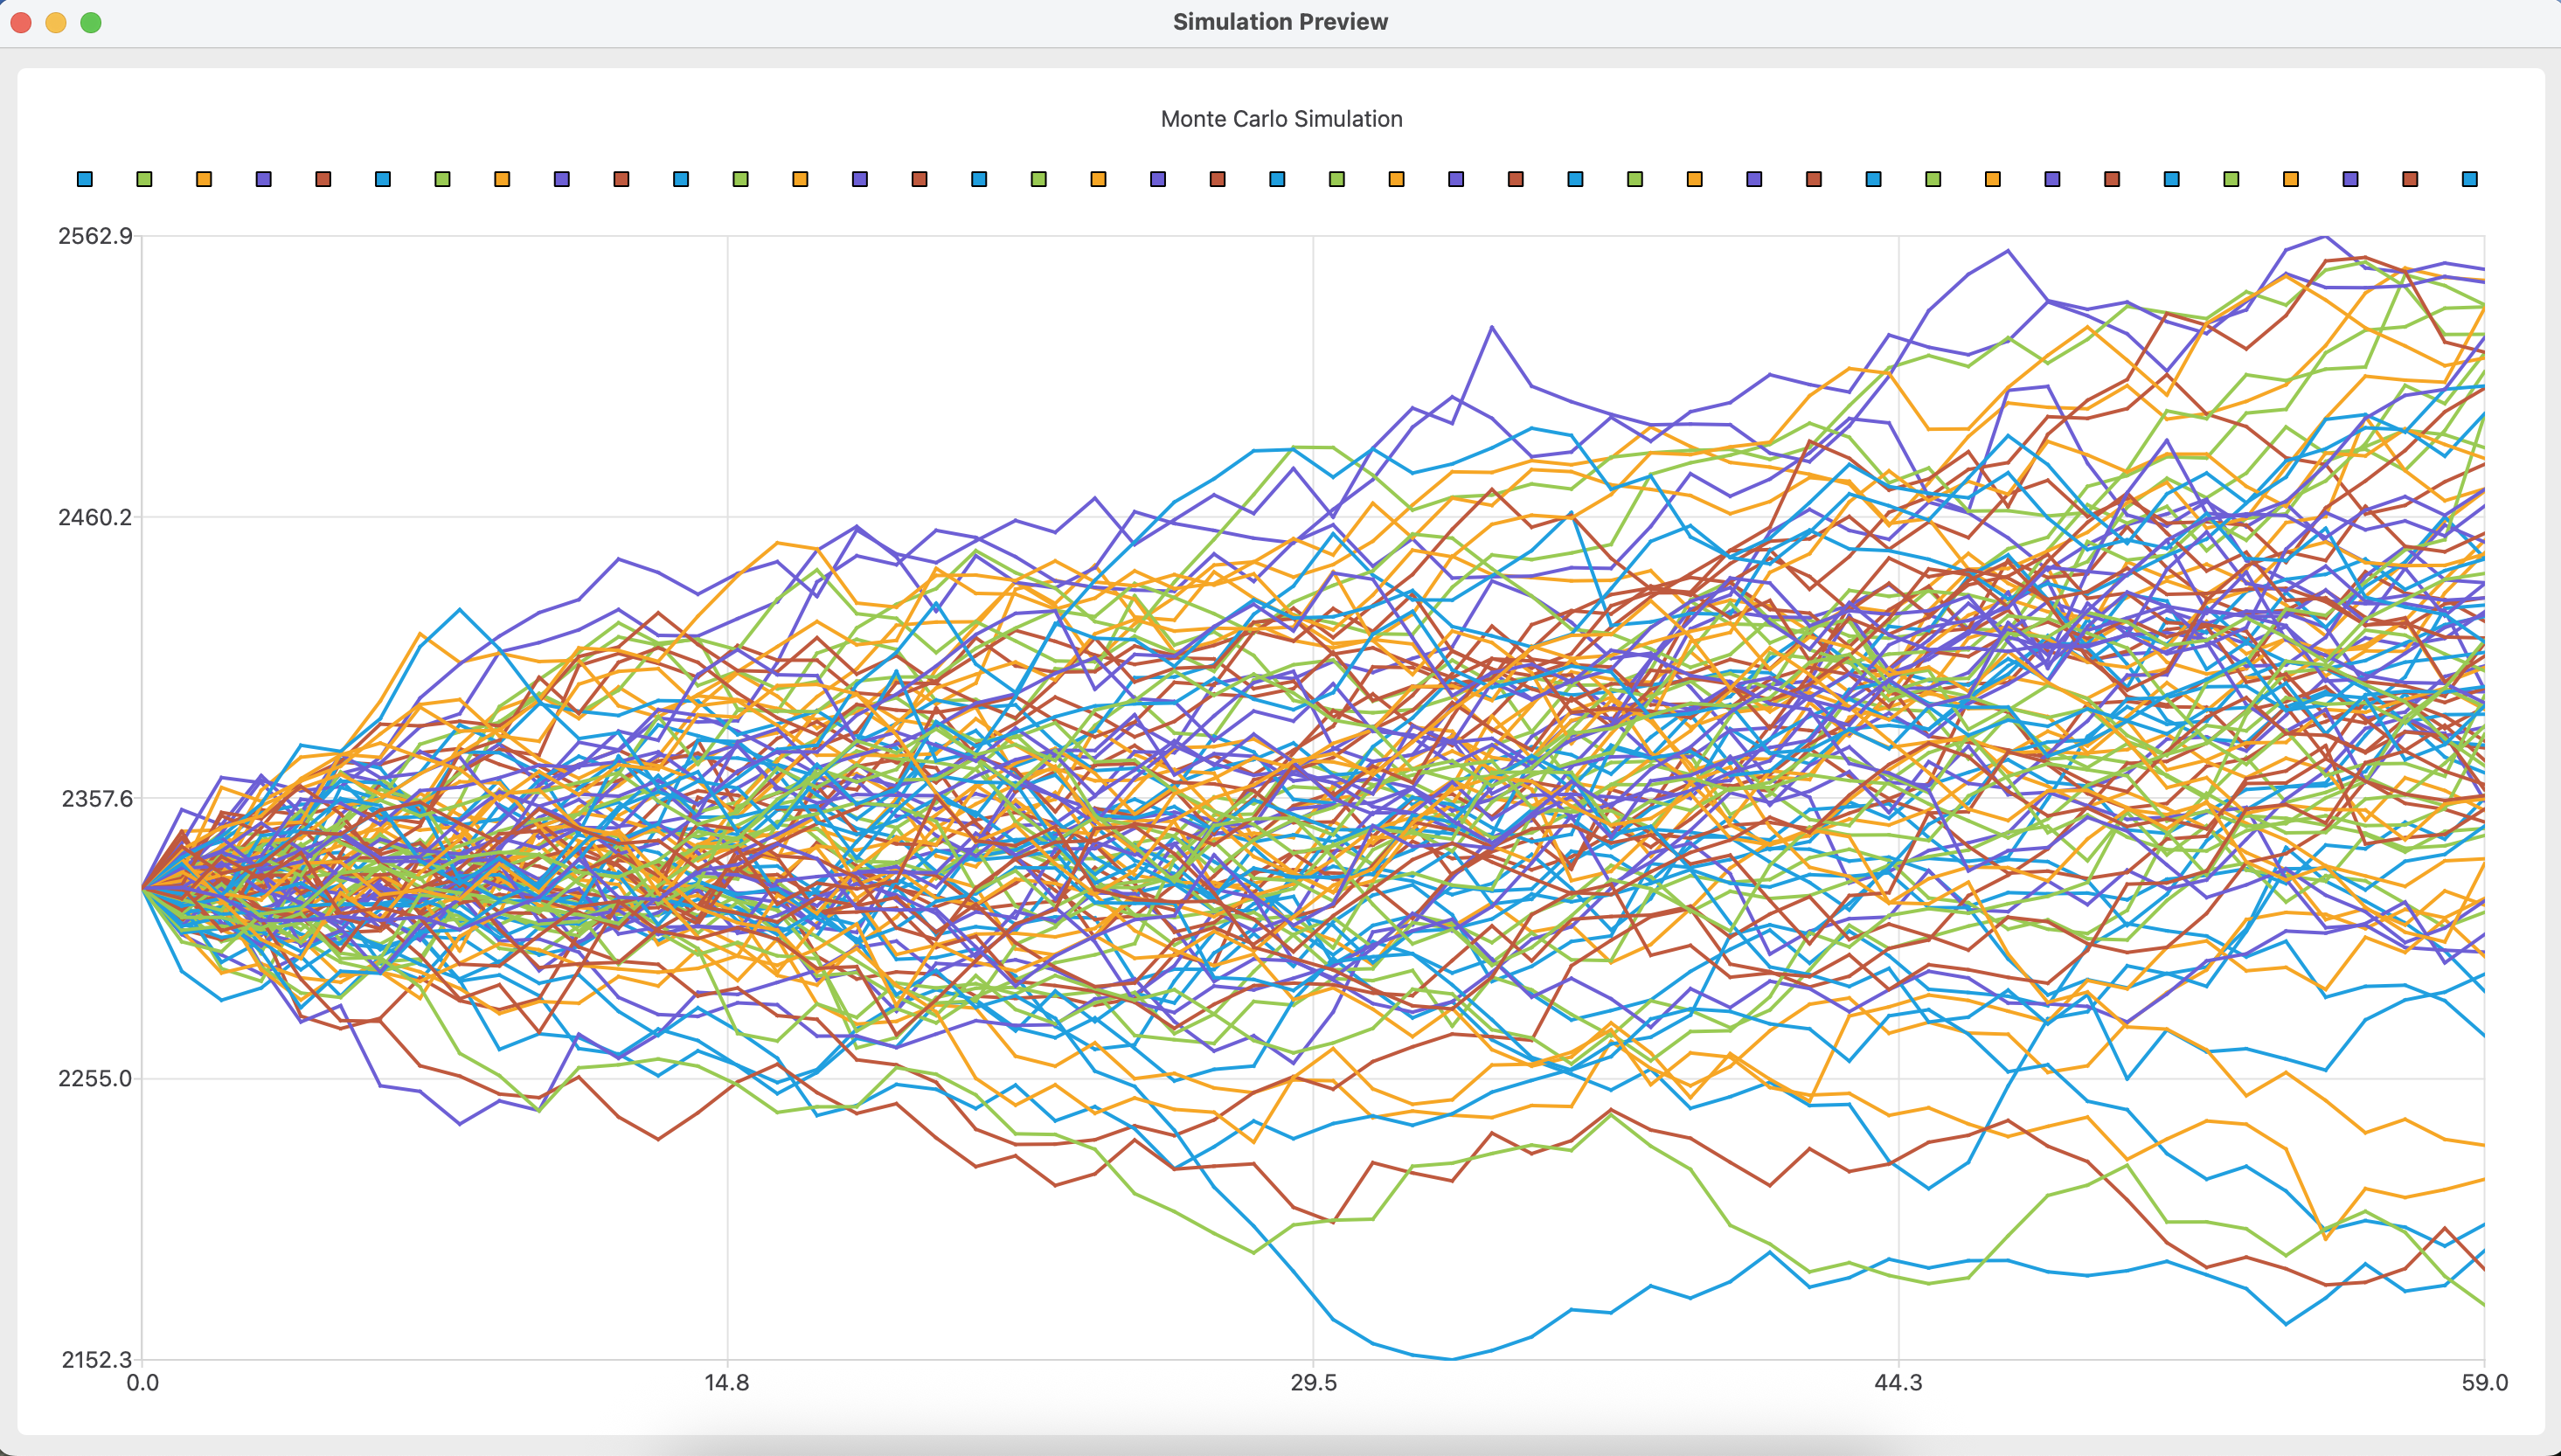
\includegraphics[width=1.5\textwidth]{Figures/monte_carlo_example.png}
    \caption{Primjer Monte Carlo simulacije portfelja kriptovaluta (100
    simulacija, 60 dana)}
    \label{fig:monte_carlo_example}
\end{figure}

\subsection{PCA dekompozicija}
\label{sek:pca_dekompozicija}
PCA dekompozicija je također implementirana kao metoda klase
\texttt{Portfolio} koja prima ulaznu kovarijacijsku matricu,
broj glavnih komponenti i vektor u koji se spremaju glavne komponente
poredane po količini varijance koju objašnjavaju te ukupnu varijancu (u ovom
slučaju to je suma svih vlastitih vrijednosti) i varijancu objašnjenu glavnim
komponentama. Metoda vrati \texttt{int} koji označava uspješnost dekompozicije.
Za izračun glavnih komponenti koristi se svojstvena dekompozicija koja
daje vlastite vrijednosti i vlastite vektore kovarijacijske matrice te je
objašnjena u \ref{sek:svojstvena_dekompozicija}.
primjer rezultata PCA dekompozicije je dan na slici
\ref{fig:pca_example}.
\begin{figure}[ht]
    \centering
    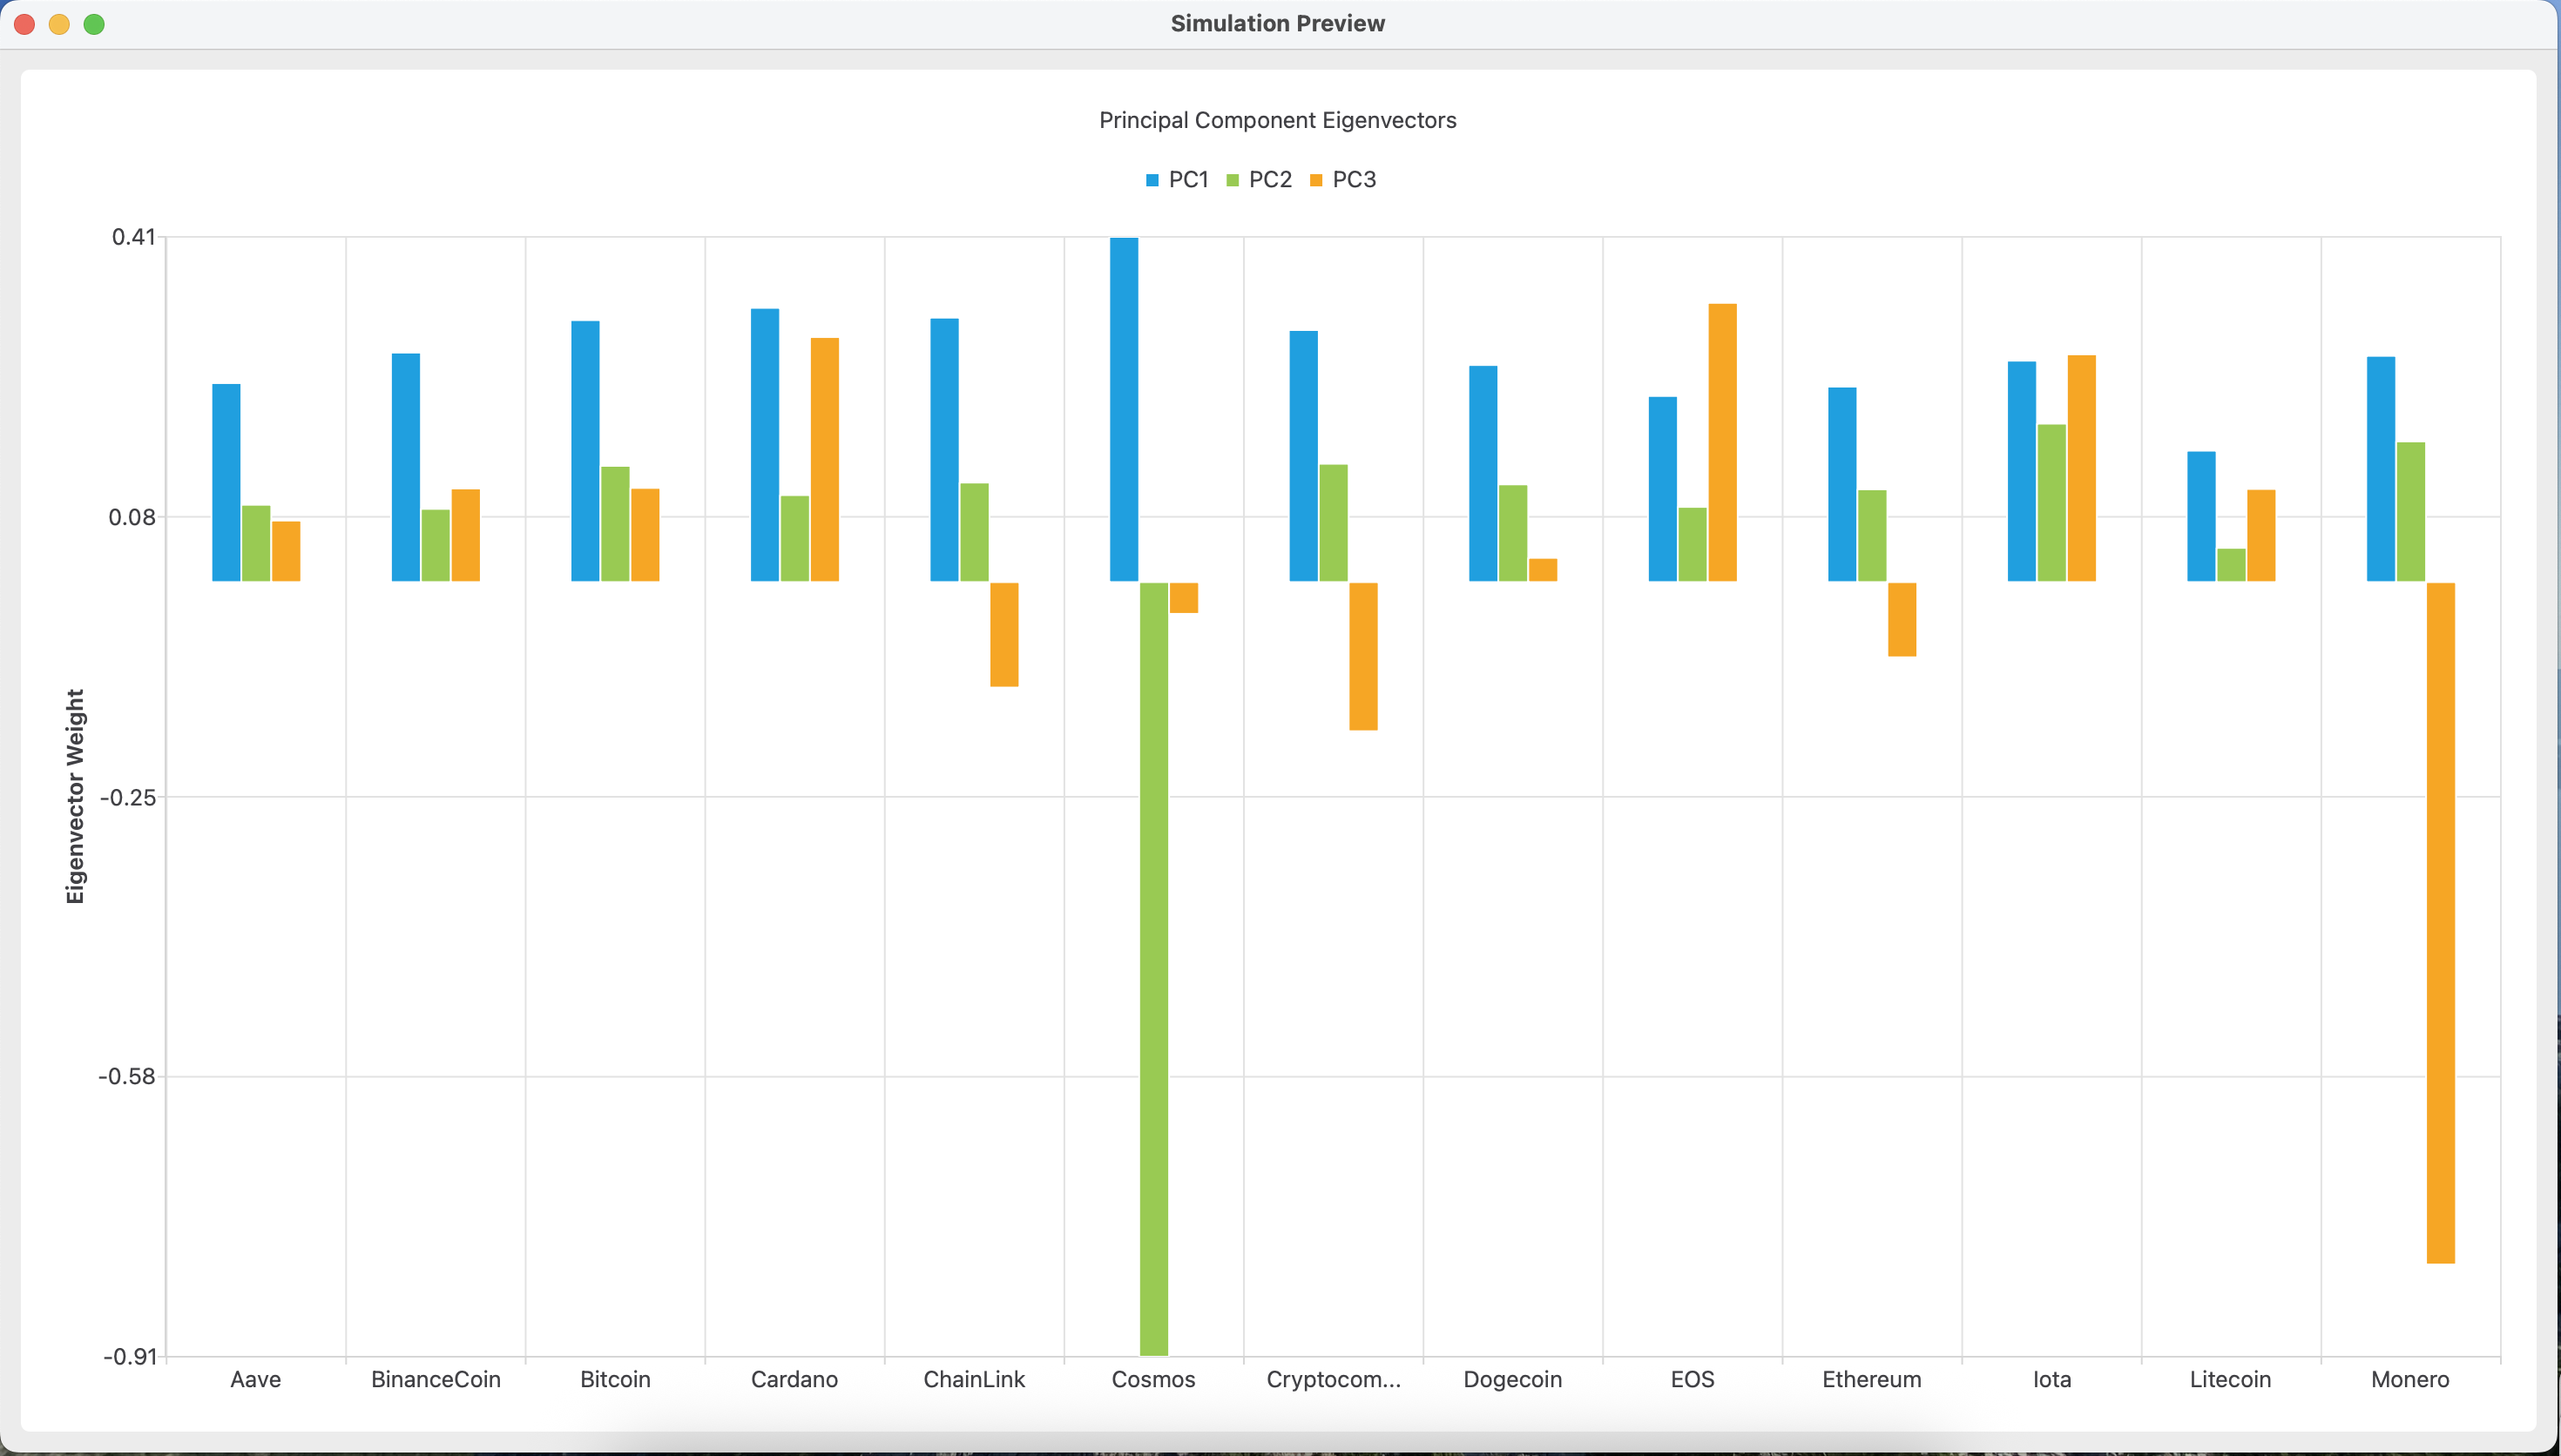
\includegraphics[width=1.5\textwidth]{Figures/pca_example.png}
    \caption{Primjer PCA dekompozicije portfelja kriptovaluta (3 glavne komponente)}
    \label{fig:pca_example}
\end{figure}

\subsection{Vizualizacija rezultata}
\label{sek:vizualizacija_rezultata}
Za vizualizaciju rezultata i interakciju s korisnikom koristi se
grafičko sučelje implementirano u C++ koristeći Qt biblioteku.
Grafičko sučelje omogućuje korisniku da odabere kriptovalute koje želi
staviti u portfelj, postavi udjele kriptovaluta u portfelju,
odabere vremenski period simulacije i broj simulacija.
Rezultati simulacija se prikazuju u obliku grafova koji
se otvaraju u novom prozoru aplikacije i prikazuju teoretsko kretanje
vrijednosti portfelja u budućnosti. Korisnik također može odabrati
broj glavnih komponenti te izvrši PCA dekompoziciju portfelja. Prikaz
rezultata PCA dekompozicije je također u obliku grafova koji
se otvara u novom prozoru aplikacije i prikazuje glavne komponente
portfelja te varijancu koju objašnjavaju.
\begin{figure}[ht]
    \centering
    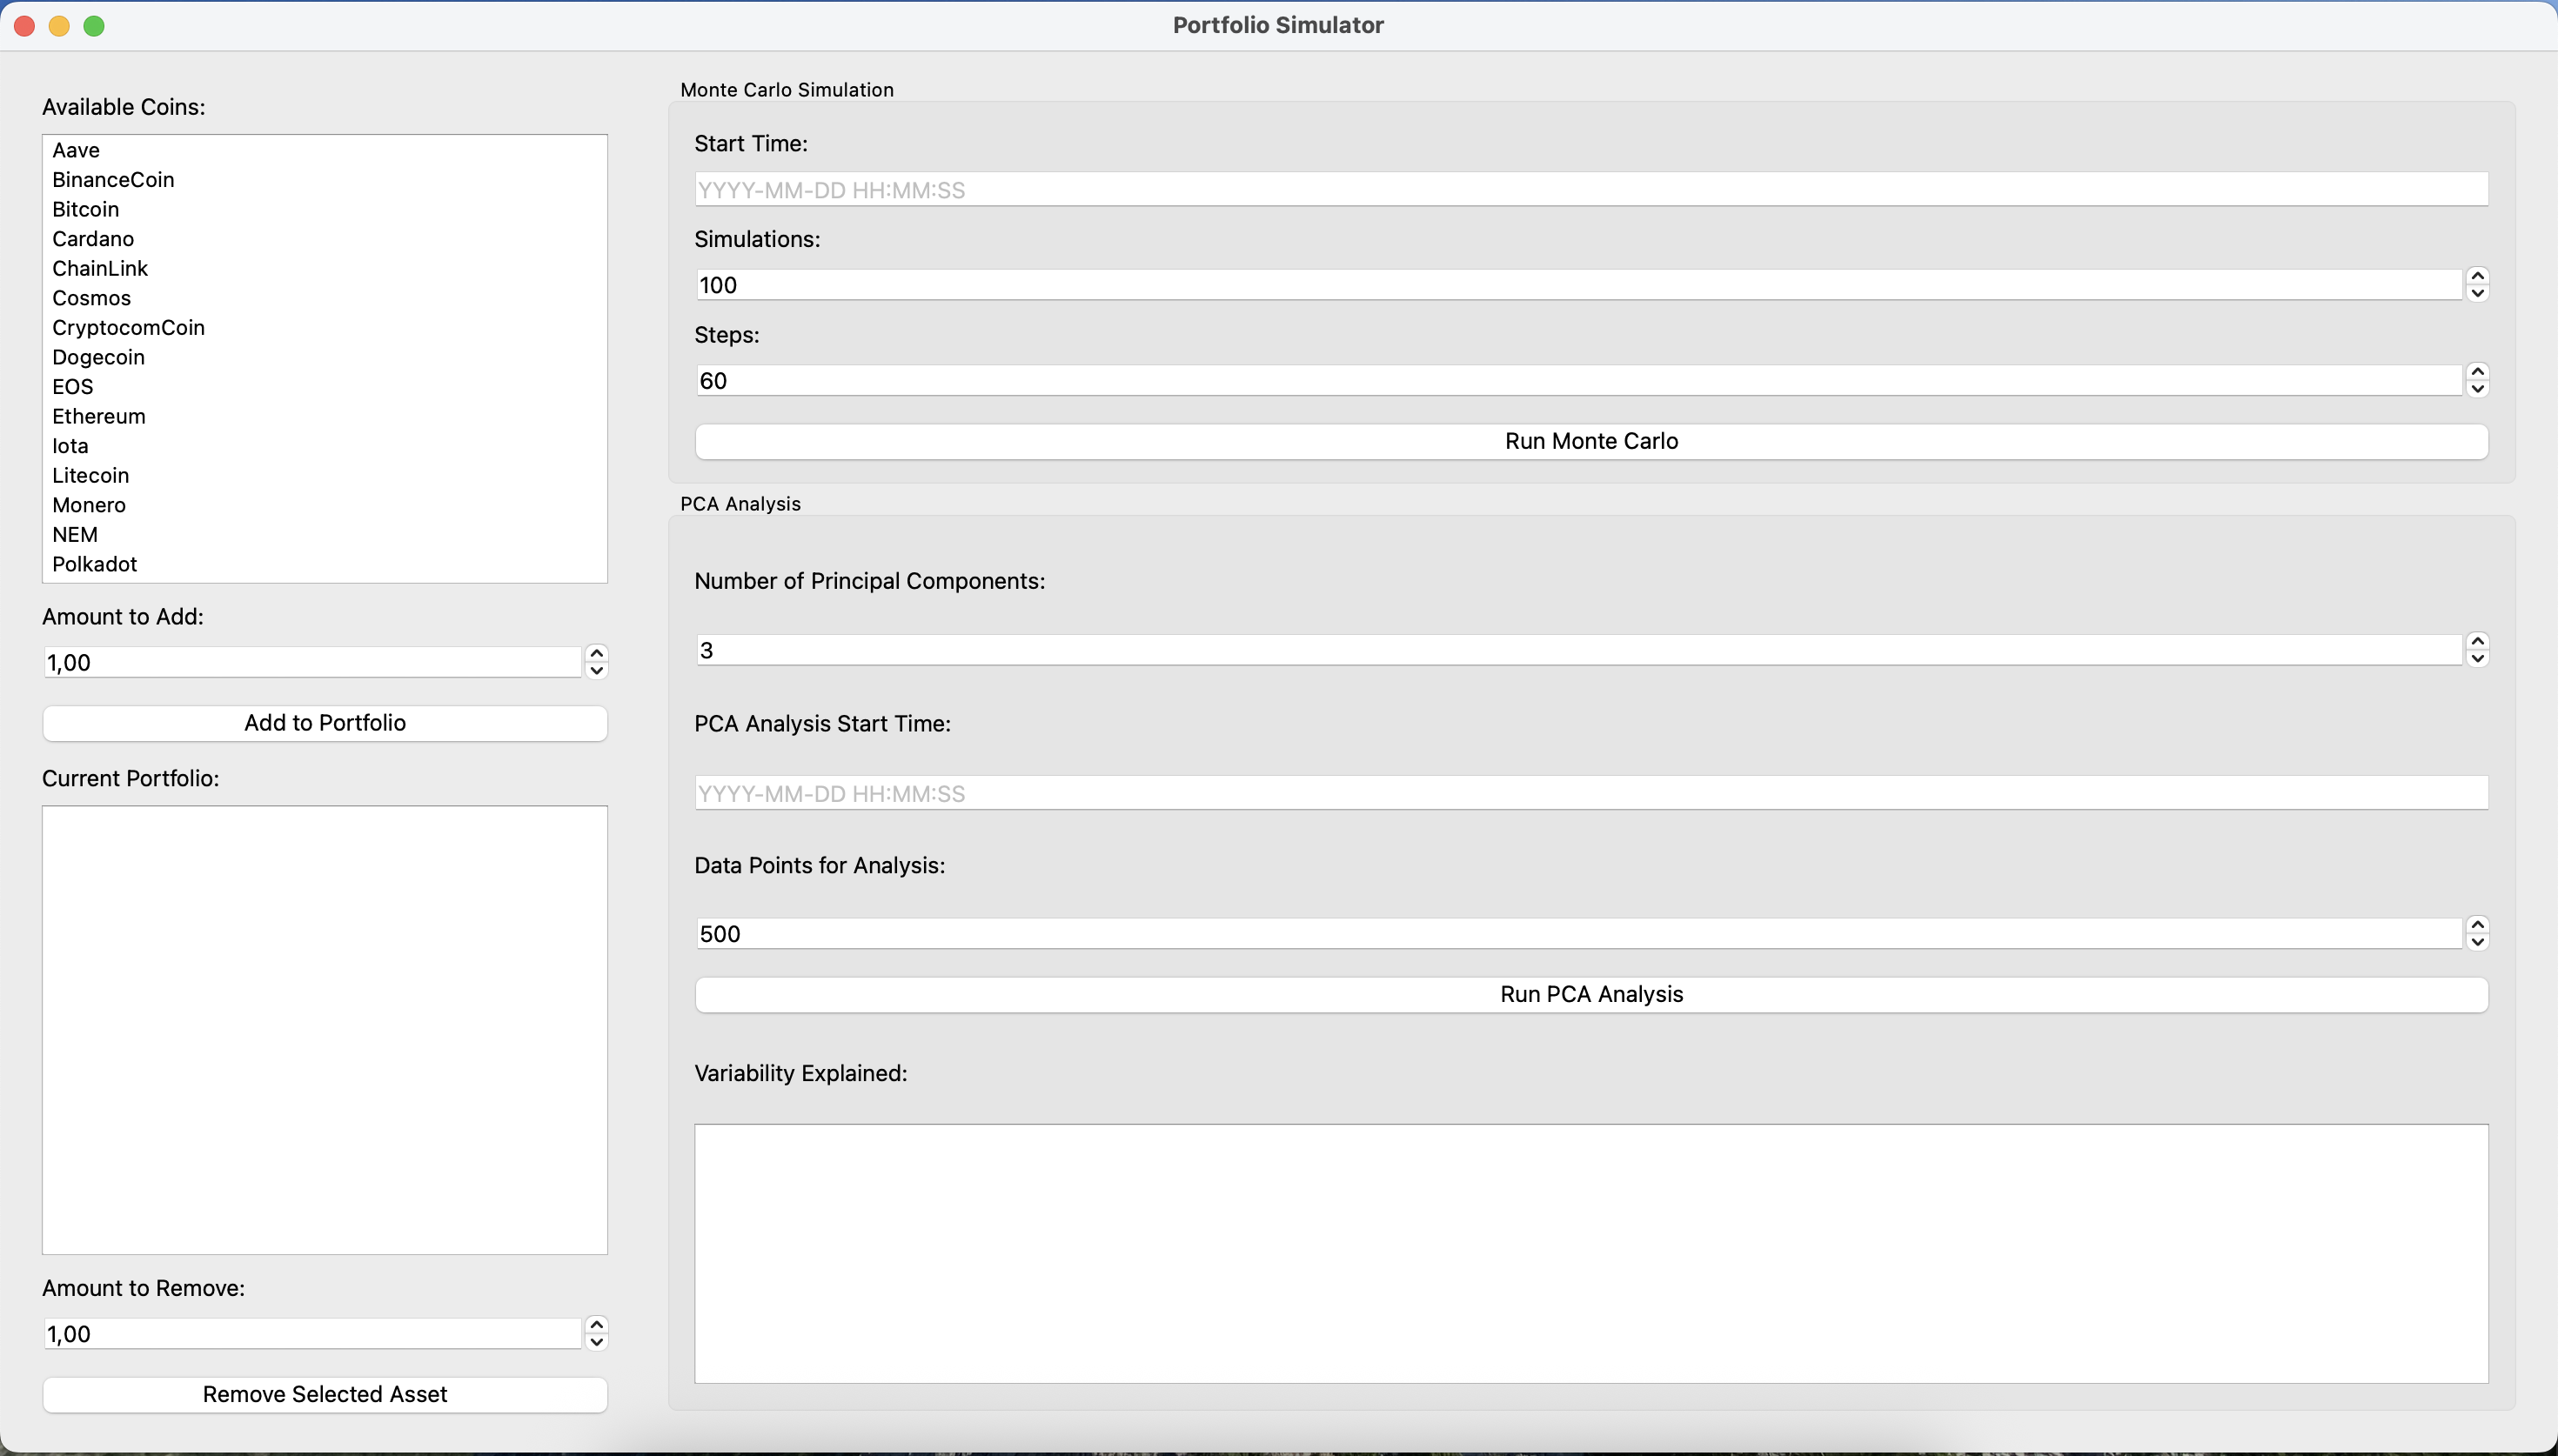
\includegraphics[width=0.8\textwidth]{Figures/gui.png}
    \caption{Grafičko sučelje aplikacije za simulaciju portfelja kriptovaluta}
    \label{fig:portfolio_gui}
\end{figure}















% Rasprava
\chapter{Rezultati i rasprava}
\label{pog:rezultati_i_rasprava}

\Blindtext

%--- ZAKLJUČAK / CONCLUSION ----------------------------------------------------
\chapter{Zaključak}
\label{pog:zakljucak}

\blindtext

%--- LITERATURA / REFERENCES ---------------------------------------------------

% Literatura se automatski generira iz zadane .bib datoteke / References are automatically generated from the supplied .bib file
% Upiši ime BibTeX datoteke bez .bib nastavka / Enter the name of the BibTeX file without .bib extension
\bibliography{literatura}

%--- SAŽETAK / ABSTRACT --------------------------------------------------------

% Sažetak na hrvatskom
\begin{sazetak}
	Unesite sažetak na hrvatskom.

	\blindtext
\end{sazetak}

\begin{kljucnerijeci}
	prva ključna riječ; druga ključna riječ; treća ključna riječ
\end{kljucnerijeci}

% Abstract in English
\begin{abstract}
	Enter the abstract in English.

	\blindtext
\end{abstract}

\begin{keywords}
	the first keyword; the second keyword; the third keyword
\end{keywords}

%--- PRIVITCI / APPENDIX -------------------------------------------------------

% Sva poglavlja koja slijede će biti označena slovom i riječi privitak / All following chapters will be denoted with an appendix and a letter
\backmatter

\chapter{The Code}

\Blindtext

\end{document}
